% CVPR 2026 Paper Template; see https://github.com/cvpr-org/author-kit

\documentclass[10pt,twocolumn,letterpaper]{article}

%%%%%%%%% PAPER TYPE  - PLEASE UPDATE FOR FINAL VERSION
\usepackage[review]{cvpr}      % To produce the REVIEW version
% \usepackage{cvpr}              % To produce the CAMERA-READY version
% \usepackage[pagenumbers]{cvpr} % Final formatting with page numbers (arXiv/turn-in)

% Import additional packages in the preamble file, before hyperref
\input{preamble}

\definecolor{cvprblue}{rgb}{0.21,0.49,0.74}
\usepackage[pagebackref,breaklinks,colorlinks,allcolors=cvprblue]{hyperref}

%%%%%%%%% PAPER ID  - PLEASE UPDATE
\def\paperID{*****} % *** Enter the Paper ID here
\def\confName{CVPR}
\def\confYear{2026}

%%%%%%%%% TITLE
\title{Unsupervised 3D Masked-Autoencoder for Coastal Ocean Anomaly Detection}

\author{Anson Chen\\
Paul G.\ Allen School of Computer Science \& Engineering\\
University of Washington, Seattle, WA 98195\\
{\tt\small ac283@uw.edu}}

\begin{document}
\maketitle

%================================================================
\begin{abstract}
Signs of harmful algal blooms along the U.S.\ Pacific Northwest coast are visible in satellite imagery, but predicting downstream biology from single channels like chlorophyll-a has worked poorly. We train a 3D convolutional masked-autoencoder on 22 years (2003--2024) of MODIS Aqua imagery over the 41--49\textdegree\,N coastal box. It takes four ocean channels (chlorophyll-a, water clarity, fluorescence, sea-surface temperature) over a 4-day window, sees no bloom labels, and produces one unsupervised ``anomaly score'' per region per day from its reconstruction error. We evaluate the score on three independent checks. At a 7-day horizon it is the only method we tested with positive $R^2$ in every region (0.10--0.26), while a matched-complexity PCA baseline sits at zero. The score for the region containing the NEMO mooring tracks in-situ \textit{Pseudo-nitzschia} cell density measured there during 2016--2018 (Spearman $\rho{=}{+}0.28$, $p{=}0.02$; Pearson $r{=}{+}0.46$) though the particulate-toxin signal is weaker. Its summer-mean score for 2014 is the highest on record in three of four regions, matching the documented Pacific marine heatwave.
\end{abstract}

%================================================================
\section{Introduction}
\label{sec:intro}

Toxin-producing \textit{Pseudo-nitzschia} blooms happen every year along the U.S.\ Pacific Northwest (PNW) coast. The toxin they make, domoic acid, builds up in razor clams and shuts down beach harvests \cite{Trainer2009,McCabe2023}. These blooms are not completely invisible from space, since MODIS Aqua sees the elevated chlorophyll and the warmer-than-average water. The problem is that picking out which patches of green water will actually produce toxin from those satellite channels has historically been hard \cite{Anderson2016,Hill2020}. Blooms look different from each other, only some species produce toxin.

Single MODIS pixels near the beach are noisy, since clouds, sun glint, river plumes, and shallow-water effects all corrupt the signal. The intuition behind this work is that a per-region aggregate should be cleaner than any one pixel, and that a model can learn which spatial and channel structures to aggregate over, rather than just averaging chlorophyll. Masked autoencoders \cite{He2022MAE} are a self-supervised approach where the model has to fill in chunks of the image that have been hidden, and in natural images this forces it to learn higher-level structure than just local texture. We adapt that idea to coastal satellite imagery, where the signal is biophysical (chlorophyll, temperature) rather than categorical (cat vs.\ dog).

We call the resulting system Ocean Anomaly Detection (OAD). Our contributions are:

\begin{enumerate}\itemsep1pt
    \item A 3D convolutional masked-autoencoder that turns the MODIS cube into one daily score per coastal region.
    \item A lead-time evaluation against matched-complexity PCA and day-of-year climatology baselines, isolating the horizon at which the score's forecast skill is real rather than an artifact of composite overlap.
    \item Validation against independent in-water ESP measurements at the NEMO mooring (2016--2018), a biological signal the model never trained on.
    \item Evidence that the score recovers documented PNW climate structure, including the 2014 marine heatwave, with no event labels.
\end{enumerate}

%================================================================
\section{Related Work}
\label{sec:related}

Operational monitoring has used satellite chlorophyll-a as a near-real-time bloom indicator for coastal HABs \cite{McKibben2015}, but in PNW coastal water the relationship between chl-a and beach-level toxin outcomes is weak \cite{Trainer2000,Trainer2009}. Multi-channel approaches that combine SST, fluorescence, and clarity perform incrementally better \cite{Anderson2016}, but the per-pixel single-day framing remains limiting.

In Earth observation, SatMAE \cite{Cong2022SatMAE} applies the masked-autoencoder principle \cite{He2022MAE} to multi-spectral satellite imagery for land-cover classification, and self-supervised pretraining is now a broad subfield of remote sensing \cite{Wang2023MAE}. We adapt it to a 3D (time-augmented) coastal ocean cube, where the temporal axis lets the model learn dynamics as well as spatial structure.

The Environmental Sample Processor \cite{Scholin2017} is an autonomous in-water sampler deployed at the NEMO mooring during ChaBa \cite{Moore2021ESP}, measuring \textit{PN} cell density and particulate domoic acid at daily cadence; these are our independent biological validation target. \cite{Moore2021ESP} finds that satellite chlorophyll-a at NEMO tracks biomass but not the elevated \textit{PN} and toxin that actually matter, which is part of why we use a multi-channel learned representation rather than a single-channel retrieval.

%================================================================
\section{Method}
\label{sec:method}

\textbf{Data.} The training cube is built from MODIS Aqua Level-3 daily ocean-color products \cite{NASA_OceanColor} covering 2003--2024 ($\sim$4{,}700 daily rolling 8-day composites) on a 321$\times$409 grid at 0.025\textdegree\ resolution. Four channels are used: chl-a, Kd490 (water clarity), normalized fluorescence (nFLH), and SST. A 2D mask excludes land pixels, and NaN pixels are excluded per-pixel from the masked-MSE reconstruction loss.

\textbf{Architecture.} OAD is a 3D ConvAE applied to $64\times64$ spatial patches tiled over the $321\times409$ grid, each of shape $(C{=}4,\, T{=}4,\, H{=}64,\, W{=}64)$ (\cref{fig:architecture}). The encoder applies three blocks of 3D convolution with stride-2 downsampling, batch normalization, and ReLU activation, reducing the $64\times64$ field to a $128{\times}1{\times}8{\times}8$ bottleneck (latent dimension 32). The decoder mirrors the encoder with transposed convolutions and upsampling.

\textbf{Training.} We train the network as a masked autoencoder \cite{He2022MAE}: a random fraction of the input pixels is hidden and the network must reconstruct them from the surrounding context, which keeps it from simply copying local texture. A plain autoencoder without masking did exactly that, and its reconstruction error tracked bloom events poorly. We hide 70\% of pixels (\texttt{mae070}) in the headline model, the only mask ratio with positive multi-step forecast skill in all five regions at the 7-day lead (\cref{sec:forecastability}).

For each daily composite at region $R$, the trained model produces a per-pixel reconstruction. We average per-pixel reconstruction error over in-region ocean pixels and z-score the result against an in-region historical distribution, producing a single scalar per (region, day). Downstream analyses use only this per-region daily scalar; the convolutional model is not run again afterward.

\begin{figure*}[t!]
\centering
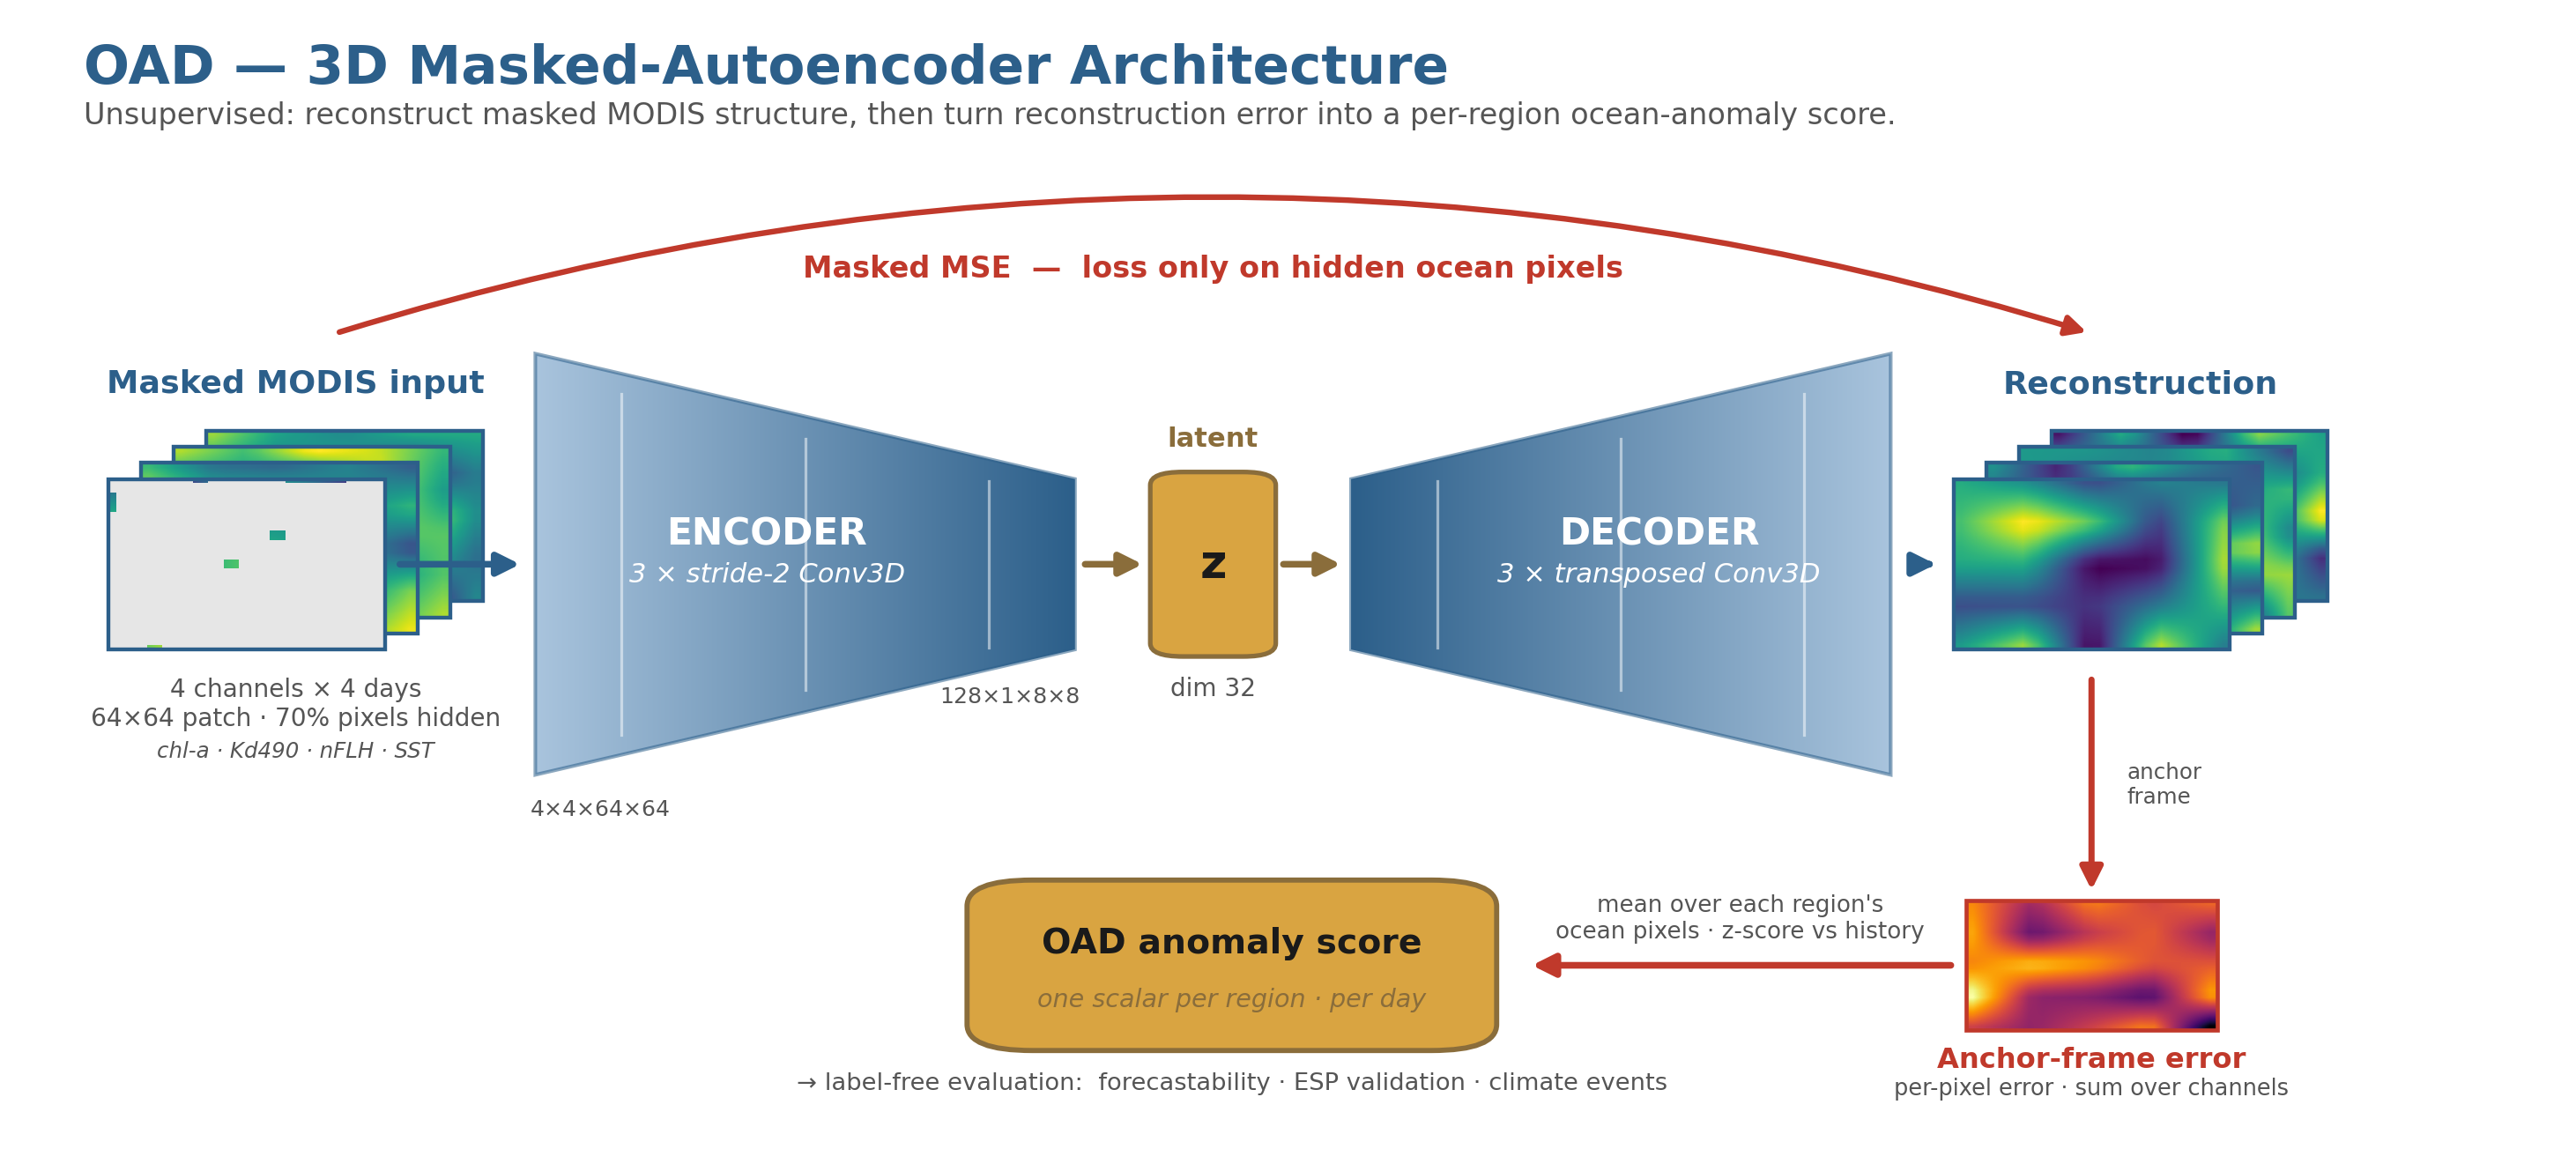
\includegraphics[width=\textwidth]{figures/fig2_architecture.png}
\caption{OAD pipeline: a 3D masked-autoencoder reconstructs a 4-channel, 4-day MODIS patch, and the per-region reconstruction error becomes the daily anomaly score.}
\label{fig:architecture}
\end{figure*}

\begin{figure}[t]
\centering
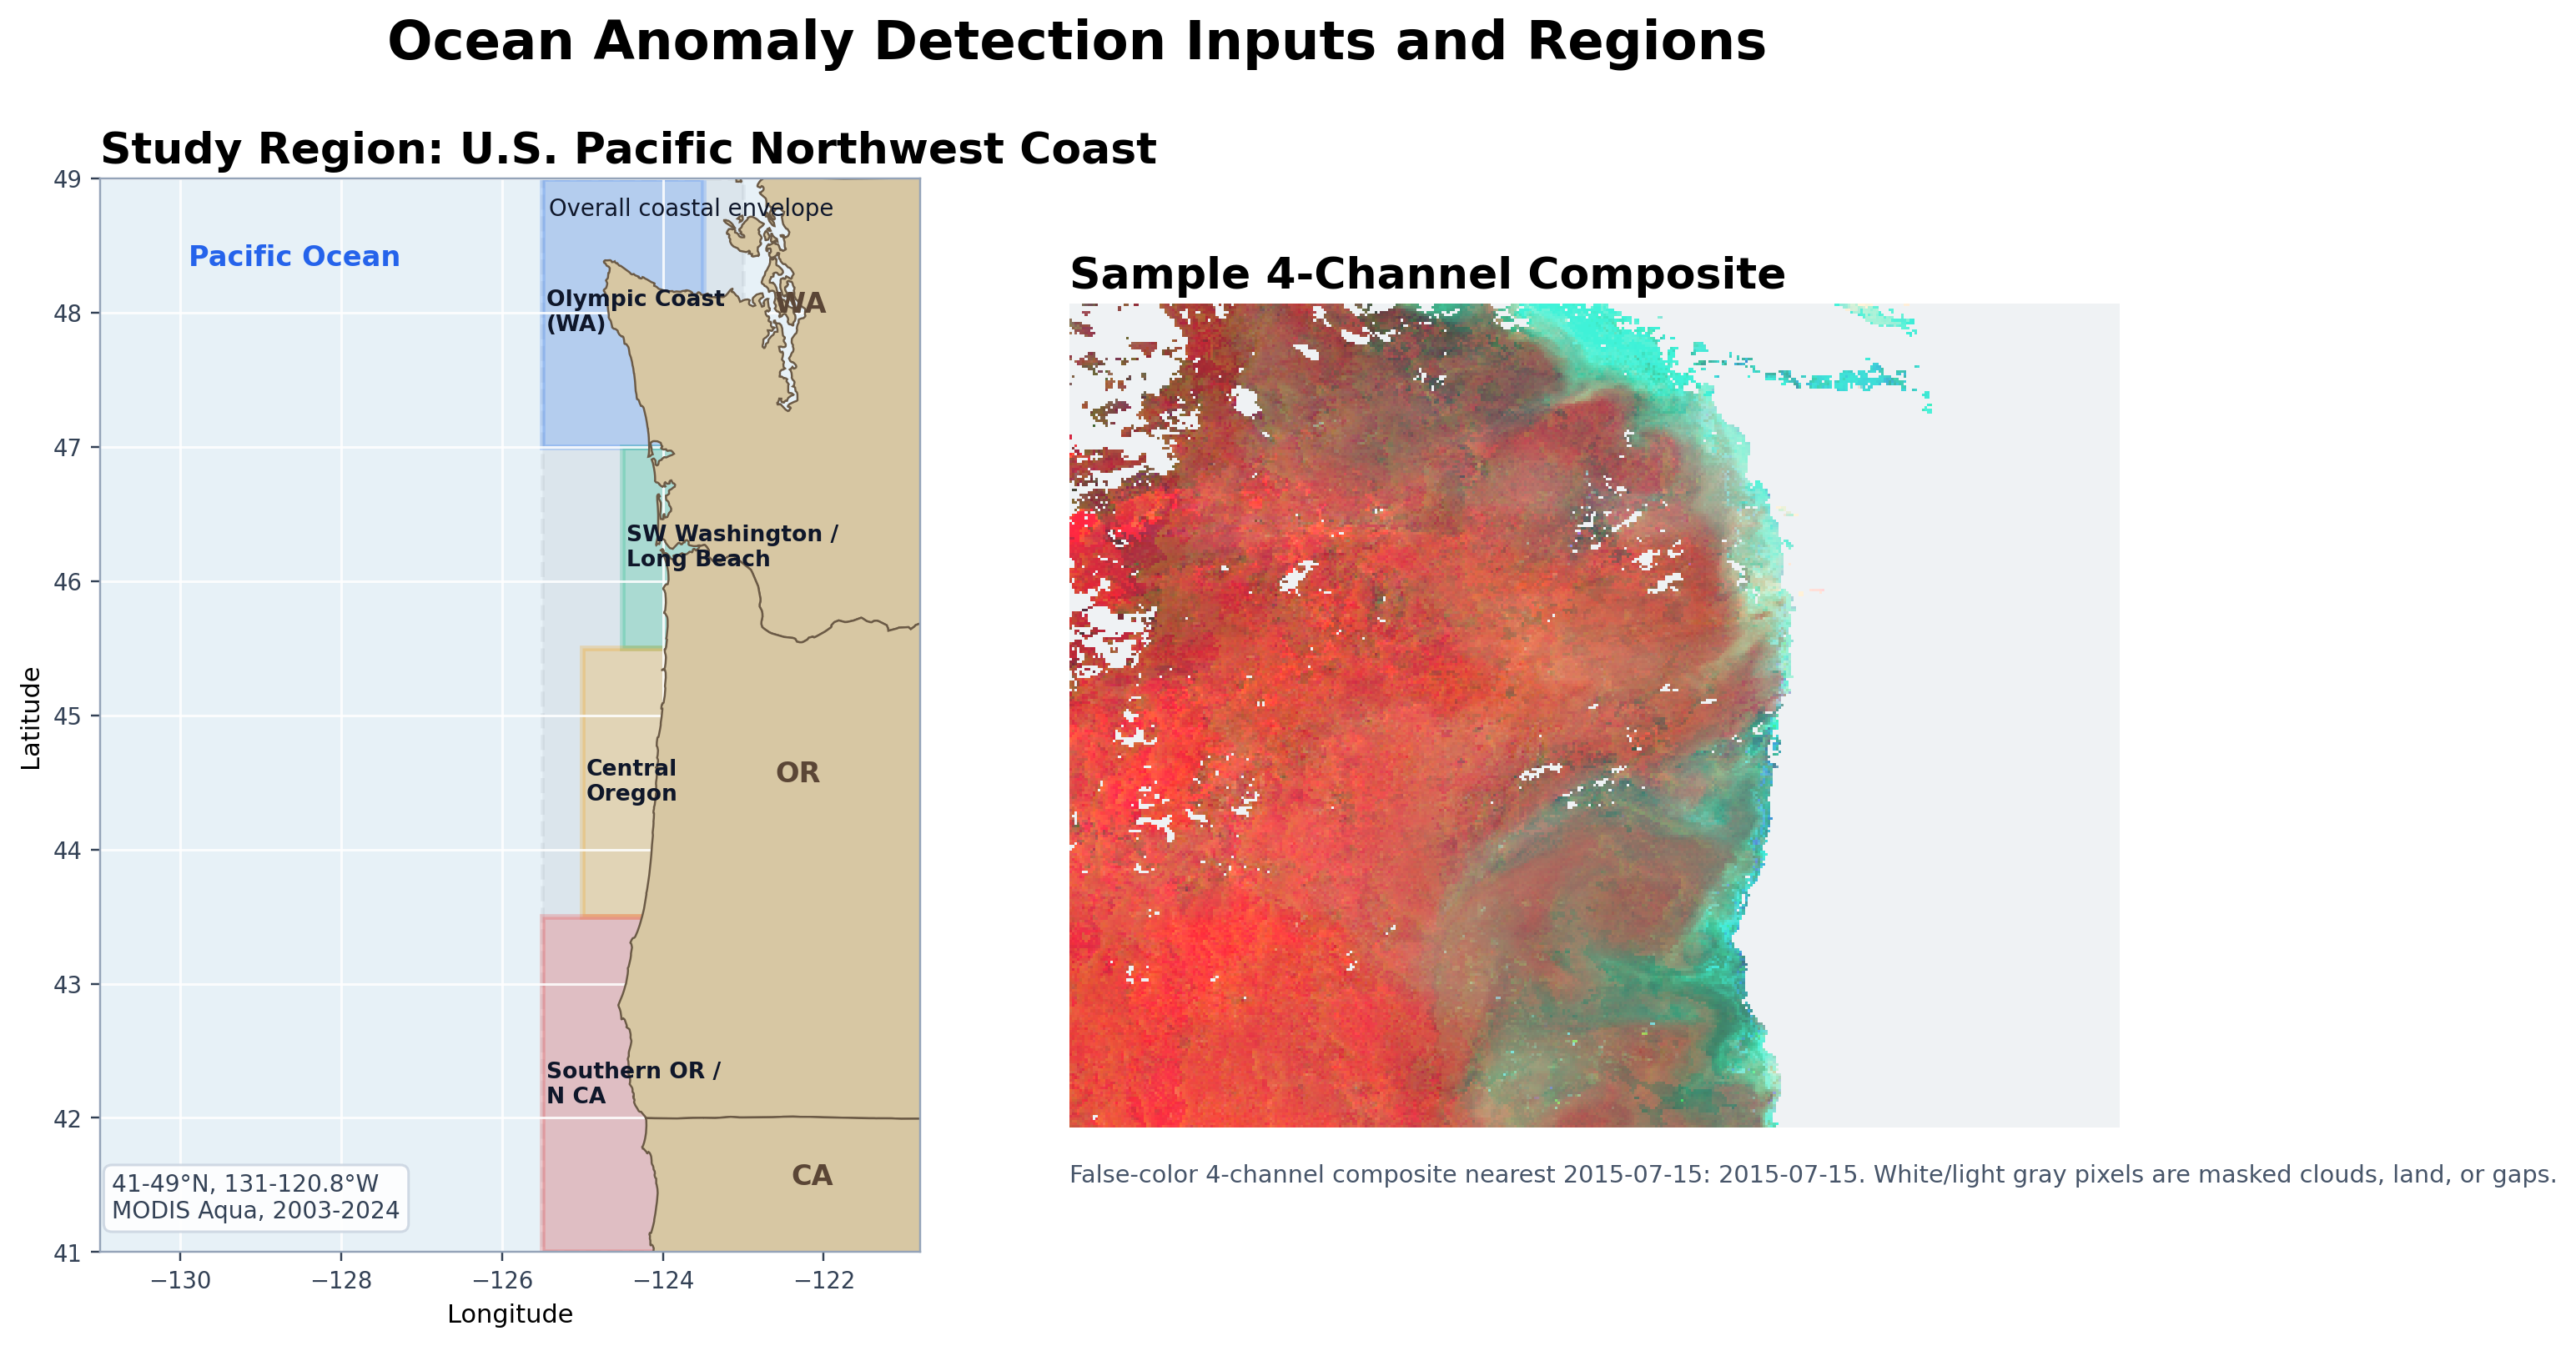
\includegraphics[width=\linewidth]{figures/fig1_study_region.png}
\caption{The U.S.\ PNW study region (41--49\textdegree\,N) with its five alongshore sub-regions and the NEMO mooring, over an example MODIS Aqua 8-day composite.}
\label{fig:study-region}
\end{figure}

%================================================================
\section{Results}
\label{sec:results}

The OAD score is evaluated in three independent ways: lead-time forecastability against baselines (\cref{sec:forecastability}), in-situ biological validation at the NEMO mooring (\cref{sec:esp}), and consistency with documented PNW climate events (\cref{sec:climatology}).

%-----------
\subsection{Lead-time forecastability vs. baselines}
\label{sec:forecastability}

We compare OAD against a matched-dimensionality PCA baseline and a day-of-year climatology baseline, forecasting per-region anomaly state from the past four days on the 2019+ held-out period. \cref{tab:leadtime} reports results for SW Washington (the highest-amplitude region), and \cref{fig:forecastability} shows the cross-region picture at the 7-day horizon.

\begin{table}[t]
\centering\small
\caption{Lead-time forecastability $R^2$, SW Washington region (2019+ held-out); the 1-day value is inflated by 8-day composite overlap.}
\label{tab:leadtime}
\begin{tabular}{lcccc}
\toprule
\textbf{Lead} & \textbf{OAD-50} & \textbf{OAD-70} & \textbf{PCA} & \textbf{Climatology} \\
\midrule
1\,day  & $+0.84$ & $+0.87$ & $-0.13$ & $+0.71$ \\
7\,days & $+0.08$ & $+0.15$ & $-0.13$ & $-0.10$ \\
14\,days & $+0.01$ & $+0.05$ & $-0.13$ & $-0.19$ \\
\bottomrule
\end{tabular}
\end{table}

At the honest 7-day lead, OAD is the only method we tested with positive $R^2$ in every one of the five PNW regions (range 0.10--0.26). PCA, with the same number of dimensions, drops to roughly zero in every region, and the day-of-year climatology baseline actively does worse than predicting the mean in most regions (\cref{fig:forecastability}). These values are low, most of next week's ocean state stays unexplained, but only OAD clears zero, while the matched-complexity baselines do not. That separation is the result here, not the absolute number.

\textbf{Does the learning matter, or is the aggregation alone enough?} The original motivation for OAD was that single coastal pixels are noisy and a per-region aggregate should be cleaner. \cref{fig:forecastability} tests this directly. The B1 baseline (gray, lightest) is the regional mean of chlorophyll-a over the same pixels OAD sees, z-scored against history, which is the ``just average chl-a over the region'' strawman. It sits at zero in every region. The B2 baseline (gray, darker) averages all four channels the same way and does \emph{worse}, because the extra channels add noise without a learned weighting. The autoencoder is supplying the ``learn what to combine'' step that simple regional averaging cannot.

\begin{figure}[t]
\centering

\includegraphics[width=\linewidth]{figures/fig3_forecastability.png}
\caption{Held-out 7-day-ahead forecast skill ($R^2$) by region (2019+): OAD (purple) is positive in all five regions, while the matched-complexity PCA and day-of-year climatology baselines are not.}
\label{fig:forecastability}
\end{figure}

%-----------
\subsection{In-situ validation against ESP/ChaBa}
\label{sec:esp}

To test whether OAD captures real biology, we compare it against independent in-situ measurements at the same place and time. We use ESP-derived \textit{PN} cell density and particulate domoic acid (pDA) from the 2016--2018 ChaBa deployments at the NEMO mooring (47.97\textdegree\,N, 124.97\textdegree\,W) \cite{Moore2021ESP}. NEMO lies within our Olympic Coast region, so we compare them against that one region's OAD score. Because cell-density and toxin distributions are heavy-tailed (a few bloom days dominate), we report both Pearson $r$ on raw values \emph{and} the rank-based Spearman $\rho$ (\cref{tab:esp}), each with a bootstrap confidence interval.

\begin{table}[t]
\centering\small
\caption{OAD score vs.\ in-situ ESP measurements at NEMO (2016--2018), with Pearson and rank-based Spearman correlations and 95\% bootstrap CIs.}
\label{tab:esp}
\setlength{\tabcolsep}{4pt}
\begin{tabular}{@{}lccc@{}}
\toprule
\textbf{Measurement} & \textbf{Pearson} $r$ & \textbf{Spearman} $\rho$ & $N$ \\
\midrule
\textit{PN} cells & $\mathbf{+0.46}$\,[.17,.66] & $\mathbf{+0.28}$\,[.01,.51] & 76 \\
pDA (toxin)       & $+0.34$\,[.02,.54]         & $+0.19$\,[$-$.03,.39]       & 90 \\
\bottomrule
\end{tabular}
\end{table}

The \textit{PN}-cell signal is the robust one. The OAD score for the NEMO region tracks measured cell density at $p = 3{\times}10^{-5}$ (Pearson) and, more conservatively, $p = 0.016$ on the rank correlation, whose bootstrap CI excludes zero (\cref{tab:esp}). As \cref{fig:esp-scatter} shows, median cell density rises monotonically across terciles of the OAD score. The particulate-toxin signal is weaker. The raw Pearson $r = 0.34$ is carried by a handful of high-toxin days, and the rank correlation is \emph{not} significant (Spearman $\rho = 0.19$, $p = 0.07$, CI spanning zero). We therefore treat \textit{PN} cell density as the validated target and pDA as a suggestive but unconfirmed secondary. The correlation is moderate and the satellite misses plenty of day-to-day biology, but because the model never trained on these in-water measurements, even this much agreement is informative.

The time-series overlay (\cref{fig:esp-ts}) shows OAD and ESP peaks tending to move together across the five 2016--2018 deployment windows. The 2017 spring deployment is the clearest case, where OAD ramps up several days before the ESP-measured \textit{PN} peak, which suggests it may be useful as a leading indicator for when to deploy in-water samplers.

\begin{figure}[t]
\centering

\includegraphics[width=\linewidth]{figures/fig5_esp_validation.png}
\caption{OAD score vs.\ in-situ biology at NEMO (2016--2018): per-day scatter (top) and median ESP value within OAD-score terciles (bottom), for cell density (left) and toxin (right).}
\label{fig:esp-scatter}
\end{figure}

\begin{figure}[t]
\centering

\includegraphics[width=\linewidth]{figures/fig9_oad_esp_timeseries_wide.png}
\caption{Daily overlay of the Olympic Coast OAD score (line) and NEMO ESP measurements (markers),\textit{PN} cells (top) and particulate domoic acid (bottom), across the five 2016--2018 ChaBa deployments (shaded).}
\label{fig:esp-ts}
\end{figure}

%-----------
\subsection{Agreement with documented PNW climatology}
\label{sec:climatology}

The unsupervised score also recovers well-established PNW coastal ocean patterns. Three stand out.

\textbf{Seasonal cycle.} The score rises sharply in late spring (April--May), peaks in mid-summer, and declines through autumn across all five regions, matching canonical PNW \textit{PN} bloom phenology \cite{Trainer2000,Trainer2009,McKibben2017}. Amplitude is largest in SW Washington (Columbia River plume plus shelf upwelling) and Olympic Coast (the Juan de Fuca eddy retains nutrient-rich water \cite{Marchetti2004}).

\textbf{The 2014 marine heatwave stands out.} One test of the score's climate sensitivity is whether it picks out the year of the 2014--16 Pacific marine heatwave (``the Blob'' \cite{Bond2015}), which triggered the largest \textit{P.\ australis} bloom on record \cite{McCabe2016,McCabe2023}. \cref{fig:climatology-ts} plots the monthly-mean OAD score per region across 2003--2024. In Olympic Coast, Central Oregon, and Southern OR/N.\ California, 2014 is the highest summer-mean of all 19 measured years, and in SW Washington it is the second-highest. The model was never told which years had blooms, so this ranking comes entirely from the satellite imagery itself.

\textbf{Regions move together but keep local detail.} Regional scores correlate at $> 0.5$ on monthly means, consistent with large-scale Pacific climate drivers (PDO, ENSO) \cite{Mantua1997,Jacox2018}, but each region keeps its own short-term signal from local eddies, plumes, and wind events.

\begin{figure}[t]
\centering

\includegraphics[width=\linewidth]{figures/fig4_climatology_timeseries.png}
\caption{Monthly-mean OAD score per region (2003--2024); the shaded 2014--16 marine heatwave is the highest sustained anomaly and the gray band marks the 2009--11 MODIS coverage gap.}
\label{fig:climatology-ts}
\end{figure}

\FloatBarrier

%================================================================
\section{Discussion}
\label{sec:discussion}

Across all three checks the absolute numbers are small, but the comparisons hold. OAD is the only method that beats the mean at a 7-day lead; its NEMO cell-density correlation stays significant under a rank test against an instrument it never trained on; and it flags 2014 as the standout heatwave year with no temporal labels. None of this proves the score is a finished bloom-prediction tool. It does show that an unsupervised representation of the satellite cube picks up structure the linear baselines miss and that lines up with real biology at the source.

Per-region Pearson correlation between the OAD score and the in-region valid-pixel fraction is moderate. For our headline mae070 checkpoint, SW Washington shows $r \approx +0.49$ ($\sim$24\% of variance covaries with cloud cover) and Olympic Coast shows $r \approx +0.46$ ($\sim$21\%). The mae050 variant is 4--9 percentage points lower on this metric, the cloud half of the tradeoff weighed in \cref{sec:method}. Downstream applications should carry the in-region valid-pixel fraction as a parallel feature so consuming models can learn to discount cloudy weeks.

What this paper does \emph{not} show is whether the source-region OAD score predicts beach-level shellfish toxicity. That depends on a chain of additional physics, including wind direction, onshore transport, which \textit{PN} species is present and whether it is producing toxin, and how much each clam happens to filter. We test only the offshore signal here.

\textbf{Limitations.} (1)~the 2009--2011 MODIS coverage gap leaves wide uncertainty in some regions, (2)~the cloud-confound is partial ($\sim$21--24\% variance), (3)~in-situ validation uses only one mooring (NEMO) with 76--90 daily samples, and (4)~regions are hand-defined, so learning regions via clustering on the latent is a natural extension.

\textbf{Lessons learned.} The matched-complexity PCA baseline ended up mattering more than the autoencoder itself: without it, a positive $R^2$ reads as nothing more than ``a bigger model fits better,'' and it was the gap between the two, not OAD's absolute number, that turned out to be the result worth reporting since the result was a lot lower then I was expecting in all the various correlation. The evaluation horizon mattered as much as the metric, since the inflated 1-day score from 8-day composite overlap would have overstated everything had we stopped there instead of pushing to a 7-day lead and would've leaked data. And the cloud-cover confound only surfaced because we checked for it directly, which means its important to test a learned signal against the obvious nuisance variable before fully trusting it.

%================================================================
\section{Conclusion}
\label{sec:conclusion}

We trained an unsupervised 3D masked-autoencoder on 22 years of MODIS Aqua imagery and turned its reconstruction error into one anomaly score per coastal region per day. The score is modest but carries real signal: it is the only method we tested that beats the mean at a 7-day lead in every PNW region, it tracks in-situ \textit{PN} cell density at a mooring it never trained on, and it independently picks out the 2014 marine heatwave. Useful next steps are to learn the regions by clustering the latent instead of hand-defining them, to regress out the cloud-cover correlation, to validate against more than the single NEMO mooring, and to test whether the offshore score, combined with onshore-transport physics, adds skill to beach-level toxicity forecasts, the question this paper deliberately leaves open.


{\small
\bibliographystyle{ieeenat_fullname}
\bibliography{references}
}

\end{document}
